\documentclass[runningheads,a4paper]{llncs} \usepackage[utf8]{inputenc}
\usepackage[hyphens]{url}
\usepackage{graphicx}
\usepackage{hyperref}
\usepackage{float}
\usepackage{eurosym}
\usepackage[normalem]{ulem}
\usepackage{alltt}
\usepackage{subfig}
\usepackage{amssymb}
\setcounter{tocdepth}{3}

\usepackage{url}
\newcommand{\keywords}[1]{\par\addvspace\baselineskip
\noindent\keywordname\enspace\ignorespaces#1}

\begin{document}

\mainmatter  % start of an individual contribution

% first the title is needed
\title{Context-aware Querying for\\ Multimodal Search Engines}

% a short form should be given in case it is too long for the running head
\titlerunning{Context-aware Querying for Multimodal Search Engines}

\author{Jonas Etzold\inst{1} \and Arnaud Brousseau\inst{2} \and Paul Grimm\inst{1} \and Thomas Steiner\inst{2}}

\authorrunning{Context-aware Querying for Multimodal Search Engines}
% (feature abused for this document to repeat the title also on left hand pages)

% the affiliations are given next; don't give your e-mail address unless you
% accept that it will be published
\institute{Erfurt University of Applied Sciences, Germany, \email{\{jonas.etzold|grimm\}@fh-erfurt.de}
\and Google Germany GmbH, ABC-Str. 19, 20354 Hamburg, Germany,
\email{\{arnaudb|tomac\}@google.com}}

\maketitle

\begin{abstract}
Multimodal interaction provides the user with multiple modes of interacting with a system, such as gestures, speech, text, video, audio, etc. A multimodal system allows for several distinct means for input and output of data. In this paper, we present our work in the context of the \mbox{I-SEARCH} project, which aims at enabling context-aware querying of a multimodal search framework including real-world data such as user location or temperature. 

\keywords{Multimodality, Context Awareness, User Interfaces}
\end{abstract}

\section{Introduction}
The I-SEARCH project aims to provide a unified framework for multimodal content indexing, sharing, search and retrieval. This framework will be able to handle specific types of multimedia and multimodal content, namely text, 2D images, hand-drawn sketches, videos, 3D objects and audio files), but also real world information that can be used as part of queries. Query results can include any available relevant content of any of the aforementioned types. This is achieved through Rich Unified Content Annotation (RUCoD), a concept that we have introduced in~\cite{ijmis}. It becomes clear that a framework like I-SEARCH faces specific challenges user interface-wise. Not only does it have to allow for the combination of multimodal queries, but it has to do so on different devices, both desktop and mobile. This research being conducted in the context of a European research project, we have time constraints to take into account, hence, we can time-wise simply not afford to develop two UI stacks separately for desktop and mobile. We show how using newly added features in the markup language HTML  we can kill these two flies with one stone.

The remainder of this paper is structured as follows: Section~2 presents related work, Section~3 introduces our chosen methodology, split up in three sub-tasks, Section~4 goes into implementation details and presents some preliminary results, Section~5 presents an Evaluation of a user study that we have conducted, Section~6 ends the paper with an outlook on future work and provides a conclusion.

\section{Related Work}
(Jonas) \cite{nigay}

(for multimodal search interfaces)

(for multimodal interaction)
Further approaches of frameworks for multimodal interaction are described by the W3C 
Multimodal Interaction Working Group with its work-in-progress specification of the 
``Multimodal Architecture and Interfaces'' \cite{w3cMMI} which is used to define the
internal structure of this component. Nevertheless UIIFace does not rely on XML
for propagating interaction commands to interface components since JavaScript
events can be more directly used in a client-based JavaScript library for this
purpose.

Other approaches to define multimodal interaction interfaces are described by
Sreekanth \cite{sreekanth}, who uses a Monitor Agent to collect events from
different modalities and Roscher \cite{roscher}, who uses the Multi-Access
Service Platform (MASP) which implements different user interface models for
each input modality and is able to combine them to more complex multimodal user
interfaces including the synchronization of all inputs along the user interface
models. In contrast to these approaches UIIFace does not deliver any UI
components and will remove the need for an interface developer to take care of
the input modality through the unified command layer which provides practically
modality-independent interaction commands.

(for collaborational search)
In order to create an appropriate concept for collaborative search several
approaches were taken into account. Mainly the work of Morris 30 and Pickens
31 described interesting ways of collaborative search approaches.  They make
use of a search session and state variables in user profiles to transfers
changes made in the interface of one user to all other collaborating users and
vice versa. Further the survey about collaborative web search practices done by
Morris 32 as well as the status quo practices presented by Amershi 15 have
influenced the decisions made during the design process of this concept. Other
approaches which mainly focus on local collaboration are described in 33 34
35. Since they mainly focus on table top interfaces and are not usable across
more than one device, those approaches were found to be not relevant to create
the Collaborative Search concept.

\section{Methodology}
In this Section we present our methodology for context-aware querying for multimodal search engines, split up in three sub-tasks \emph{MMBag}, \emph{UIIFace}, and \emph{CoFind}.

\subsection{MMBag}
MMBag stands for Multi-Modal Bag and designates the \mbox{I-SEARCH} User
Interface. It comes with specific requirements linked with the need for users to use multiple types of input: audio files or stream, video files, 3D objects, hand drawings, real-world information such as geolocation or time, image files and of course, plain text. This part of the paper shows the approach chosen to create MMBag.

Multimodal search engines are still very experimental at the time of writing. When building MMBag, we tried to look for a common pattern in search-related actions. Indeed, MMBag remains a search interface at its core. In order for users to interact efficiently with \mbox{I-SEARCH}, we needed a well-known interface paradigm. Accross the Web, a pattern has the monopoly for search related actions:  the text field, where a user can focus, enter her query, and trigger subsequent search actions. From big Web search engines such as Google, Yahoo or Bing, to small internal search engines, the pattern stays the same. 

However, \mbox{I-SEARCH} can't directly benefit from this broadly accepted pattern, as a multimodal search engine must accept a large number of types of input at the same time: audio, video, 3D objects, sketches, etc. How can this be achieved? Some search engines, even if they don't have the need for true multimodal querying, do have the need to accept input which is not plain text.

As a first example, we consider TinEye\footnote{\url{http://www.tineye.com/}}. TinEye is a Web-based search engine that allows for query by image content (QBIC) in order to retrieve similar or related images. The interface is split in two distinct parts: one part is a text box to provide a link to a Web-hosted image, while the second part allows for direct file upload (Figure~\ref{fig:tineye-ui}). This interface is a good solution for a search engine like TinEye (image input, image output) but \mbox{I-SEARCH} will need to come with more options than that.
\begin{figure}[h!]
  \centering
    
\includegraphics[width=0.8\linewidth]{resources/tineye-UI.png}
  \caption{Extract from the TinEye User Interface}
  \label{fig:tineye-ui}
\end{figure}

As a second example, we examine MMRetrieval\footnote{\url{http://www.mmretrieval.net}}~\cite{mmretrieval}. It is an attempt at bringing together image and text search to compose a multimodal query. MMRetrieval is a good showcase for the problem of designing a user interface (UI) with many user-tweakable options. For a user from outside the Information Retrieval field, the UI seems not necessarily clear in all detail, especially when specific terms such as \emph{Image ARF} are used (Figure~\ref{fig:mmretrieval-ui}).

\begin{figure}[h!]
  \centering
    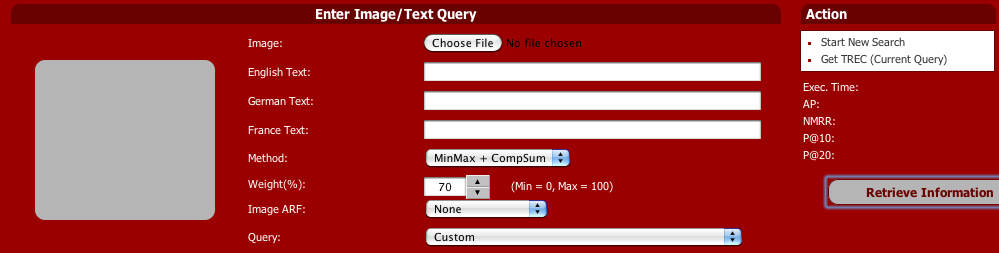
\includegraphics[width=0.8\linewidth]{resources/mmretrieval-UI.png}
  \caption{Extract from the MMRetrieval User Interface}
  \label{fig:mmretrieval-ui}
\end{figure}

Finally, we have a look at Google Search-by-image, a functionality launched on June, 14, 2011\footnote{\url{http://googleblog.blogspot.com/2011/06/knocking-down-barriers-to-knowledge.html}} and has the same requirements as MMRetrieval in terms of user interface, i.e., combining text and image input. With the Search-by-image interface, Google has succeeded in keeping the text box pattern (Figure~\ref{fig:search-by-image-box}), while preventing any extra visual noise. The interface is \emph{progressively disclosed} to users via a contextual menu when the camera icon is clicked (Figure~\ref{fig:search-by-image-popup}).

\begin{figure}[h!]
  \centering
    
\includegraphics[width=0.8\linewidth]{resources/search-by-image-UI-box.png}
  \caption{Input for the Search-by-image UI}
  \label{fig:search-by-image-box}
\end{figure}

\begin{figure}[h!]
  \centering
    
\includegraphics[width=0.8\linewidth]{resources/search-by-image-UI-popup.png}
  \caption{Popup for the Search-by-image UI}
  \label{fig:search-by-image-popup}
\end{figure}

Even if the Search-by-image solution seems very elegant, this is still not suitable for \mbox{I-SEARCH} since the interface would require a high number of small icons: camera, 3D, geolocation, audio, video, etc.  As a result, we decided to adapt a solution that can be seen in Figure~\ref{fig:isearch-ui}. This interface keeps the idea of a single text box. It is enriched by auto-completion as well as ``tokenization". The term ``tokenization" refers to the process of representing an item (picture, sound, etc.) with a small token in the text field, as if it was part of the text query. We also kept the idea of progressive disclosure for the different actions required by the various modes, e.g., uploading a picture or sketching something. The different icons are grouped together in a separated menu, close to the main search field.

\begin{figure}[h!]
  \centering
    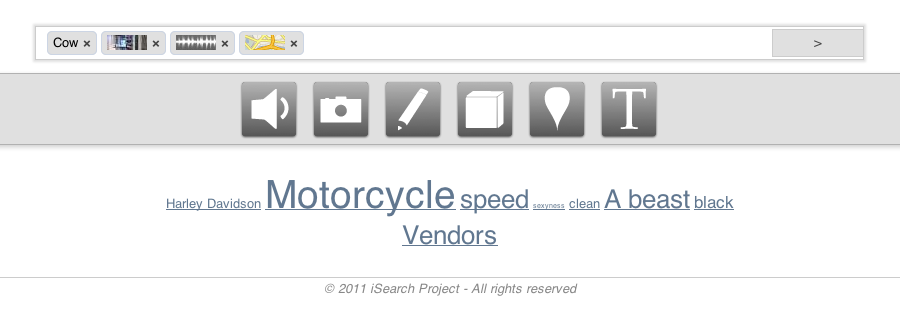
\includegraphics[width=0.8\linewidth]{resources/isearch-UI.png}
  \caption{First version of \mbox{I-SEARCH} interface}
  \label{fig:isearch-ui}
\end{figure}

\subsection{UIIFace}

Interaction is an important factor when it comes to context-awareness and
multimodality. In order to deliver a Graphical User Interface (GUI) which is
able to facilitate all the possibilities of an multimodal search engine, an
very flexible approach with a rich interaction methodology is needed. 
Further multimodal quering could also involve the way a user interacts with the
system as part of the query. 

To target all those needs the concept of UIIFace (Unified Interaction Interface)
is introduced as general interaction layer for context-arwe multimodal quering.

UIIFace describes a common interface between these interaction modalities and the 
graphical user interface (GUI) of I-SEARCH by providing a general set of interaction 
commands for the interface. Each input modality provides the implementation 
for parts of the commands or all commands defined by UIIFace. 

The idea of UIIFace is based on the OpenInterface Framework \cite{openinterface}
which describes a framework for the development of multimodal input interface
prototypes. It uses components which can represent different input modalities as
well as user interfaces and other required software pieces in order to create
and control a certain application. In contrast to this approach UIIFace is a web
implemented approach based on modern HTML5 APIs. Furthermore it provides a
command interface to web based GUIs instead of being able to create a
stand-alone application outside the browser window.

For creating the set of uni- and multimodal commands which can be used for
I-SEARCH interfaces, the results of Chang \cite{chang} as well as the needs
derived from the creation of multimodal search queries are used.

\begin{figure}[h!]
  \centering
    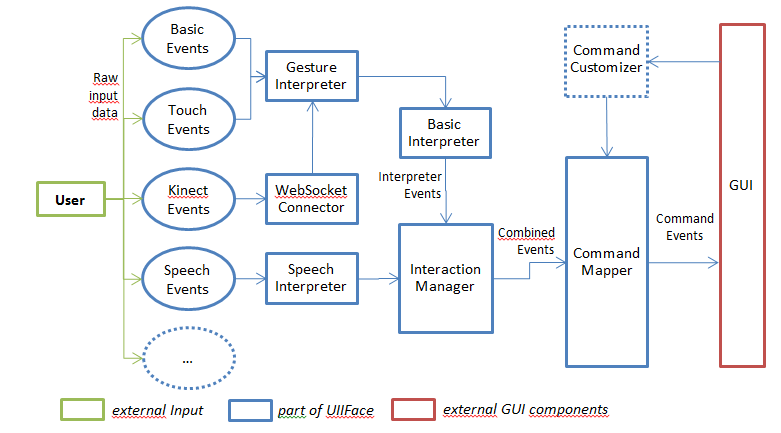
\includegraphics[width=0.8\linewidth]{resources/uiiface-structure.png}
  \caption{Schematic view on the internal structure of UIIFace}
  \label{fig:uiiface}
\end{figure}

Figure \ref{fig:uiiface} depicts the internal structure of UIIFace and shows the
flow of events. Events are raised from the users raw input. Gesture Interpreter
determines defined gestures (e.g. zoom, rotate) found in the raw input. If no
gestures were found, the Basic Interpreter routes Touch and Kinect events to
basic cursor and keyboard events. Gestures, speech commands and basic mouse,
keyboard events are then synchronized in the Interaction Manager and forwarded
as Combined Events to the Command Mapper which maps the incoming events to the
defined list of interaction commands which can be registered by any web-based
GUI. The Command Customizer can be used to rewrite the trigger event for
commands to user specific gestures or other input sequences (e.g. Keyboard
shortcuts). This is an additional feature which is not crucial to the
functionality of UIIFace but can be implemented at a later stage in order to add
more explicit personalisation features.

\subsection{CoFind}

Another part of our methodology targets the increased complexity of search
tasks and the necessity to collaborate on those tasks in order to formulate
adequat search queries which lead faster to appropriate result. The increased
complexity is primarly caused through the vast amount of unstructured data 
within the Internet and secondly through situations where the expected results
are very fuzzy or hard to describe in textual terms. 

Therefore the CoFind (Collaborative Finding) approach is introduced as an
collaborative search system which enables real-time collaborative search query
creation on a pure html website.

Likewise the collaborative approach of Google Tables and Documents -ref- the
system enables people and expert users from different domains to work together.
The main difference here is that CoFind enhances the idea of collaborative document
creation to search queries. This extension becomes even more important if
search engines allow the usage of multimodal search queries which
involve multimedia, real-world and user data in a query. 

The CoFind concept is based upon a search session concept in which HTML content
of the participants local clients is transmitted within this session.
In order to realise collaborative querying the concept provides functions for
activating collaborative search sessions, joining other online users by their
Email address and managing messaging between participants of the search session.

In general the concept consists of three main parts:
\begin{enumerate}
  \item Session Manager - controls establishment and closing of collaborative
  search sessions
  \item Content Manager - transmission of changes in user interfaces to all
  participants
  \item Messaging Manager - transmission of status and user messages to all
  participants
\end{enumerate}

Figure \ref{fig:cofind} shows how the parts of the Collaborative Search concept
interact during the search process in order to create a collaborative search session.

\begin{figure}[h!]
  \centering
    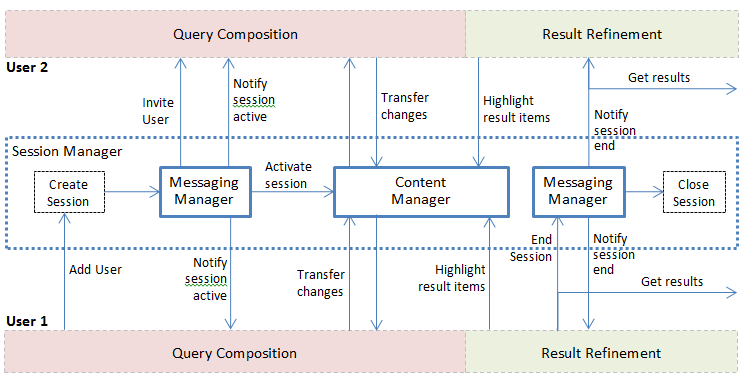
\includegraphics[width=0.8\linewidth]{resources/cofind-workflow.png}
  \caption{Schematic diagram of interaction between parts of CoFind}
  \label{fig:cofind}
\end{figure}
 
The main flow of a collaborative search session can be described as follows:
\begin{enumerate}
  \item To create or join a collaborative search session a user must supply the
  email address of the other user
  \item If other user is online and logged-in he receives an on-screen message
  and needs to accept the joining of other user
  \item after confirmation a new session entry is created which stores all
  participants
  \item every time a change on the query input field or result set is performed,
  the changed content is transferred to all participants (via WebSockets)
  \item each participant is able to navigate through the result set independent
  from others, but selections made by one user are highlighted in the result set of all other users
  \item after a user downloaded his result items or after he left the page, he
  can close the search session
\end{enumerate}

The advantages of the described concept are:
\begin{enumerate}
  \item allows collaboration on query compilation across multiple devices and
  users
  \item no interface overhead, easy to create collaborative sessions
  \item allows more precise query formulation for difficult search tasks
\end{enumerate}

\section{Implementation and Results}
(Jonas, Arnaud)

The \mbox{I-SEARCH} GUI is built using the Web platform. HTML, CSS and JavaScript are the three main building blocks for the interface. The rationale behind that choice is the following: \mbox{I-SEARCH} needs to be cross-browser and cross-device compatible. The latest specifications of those technologies enable us to do just that. Indeed, CSS3~\cite{css3}, HTML5~\cite{html5} and the therein defined new JavaScript APIs empower the browser in truly novel ways.

Our strategy also includes support for older browsers. When browsing the Web, a significant part of users don't have access to a cutting-edge Web browser. If a feature we use is not available for a certain browser version, two choices are available: either drop support for that feature if it is not important (e.g., drop visual shims like CSS shadows or border-radius), or provide alternate solution to mimic the experience. 

We would like to highlight that CSS and HTML are 2 standards that natively enable progressive enhancement thanks to a simple rule: when a Web browser doesn't understand an HTML attribute, a CSS value or selector, it simply \emph{ignores it}. This rule is the guarantee that we can build future-proof pages using CSS and HTML. Web browsers will render the page according to their capabilities: old browsers will render basic markup and styles, while modern browsers will be able to render stunning CSS3 effect.

Of course, progressive enhancement isn't always a good solution, particularly when you want to ensure that all users can access a particular feature. In this case, we will use the \emph{graceful degradation} principle, i.e, we will use fallback solutions when the technology stack is not there to support our needs in a certain browser. 

\subsection{HTML5 Semantic Markup} 

HTML5 semantic markup, with no fallback for older browsers (older browsers won't understand the extra meaning, and that's totally fine)

\subsection{CSS3 Media Queries} 

CSS3 media-queries, with Javascript fallback for older browsers

\subsection{New Javascript APIs}

 Audio, Video and File APIs, with Flash fallback

\subsection{Canvas}

\subsection{Geolocation}

\subsection{Sensors}

\subsection{Device API}


\section{Evaluation}
(Paul)
Requirement: result criteria
Did you understand the interface
Did you understand the process
2 Use Cases: Rhythm clapping (UC1) and Games (UC7)?

To validate our interface design on tasks of multimodal search we conducted a user study. 
We used a comparative study design to explore how the usage of different media types can 
influence the success rate of search queries. 

Overall, we expected that the user can handle the user interface very easily and gets a 
result which satisfies her needs. We therefore set the following hypothesis: 
\begin{enumerate}
  \item (H1) a search query will mostly contain just one modality
  \item (H2) a search refinement will be done by adding other media types
  \item (H3) a search refinement will not be done by removing query parts
  \item (H4) the use of multiple media items in a search query will result
  in faster search results compared to a single-media search
\end{enumerate}

For the user study we recruited N7N (FF,KK,TT,RR,2xGunar,Ohl) participants (NN male and NN female) aged between YYYY and YYYY. All participants were familiar with textual Web-based search. We asked all study participants to find NN different items (one audio file, one 3D model and one image, see Figure 1). All search queries are part of two uses cases which were described in section SSS. For explanation, what should be searched (and find), these items were shown in their original format to the study participants. To perform the search queries a mobile notebook with touch display was used. Consequently, for comparison with single-media search the study participants should find the same objects using common search single-media search engines. Our goal was to validate our interface design as well as to measure the impact of the possibility of multimodal search. 

All users completed all tasks successfully. As a rough measure of task performance

\section{Conclusion and Future Work}
(Tom)

\section{Acknowledgments}
This work is partly funded by the EU FP7 \mbox{I-SEARCH} project under project reference 248296.

\bibliographystyle{plain}
\bibliography{mmm2012}
\end{document}
